\section{Microcomputer Organization}
\subsection{Base Microcomputer Structure}

    \begin{wrapfigure}{R}{5cm}%TODO WO??
        \vspace{-1cm}
        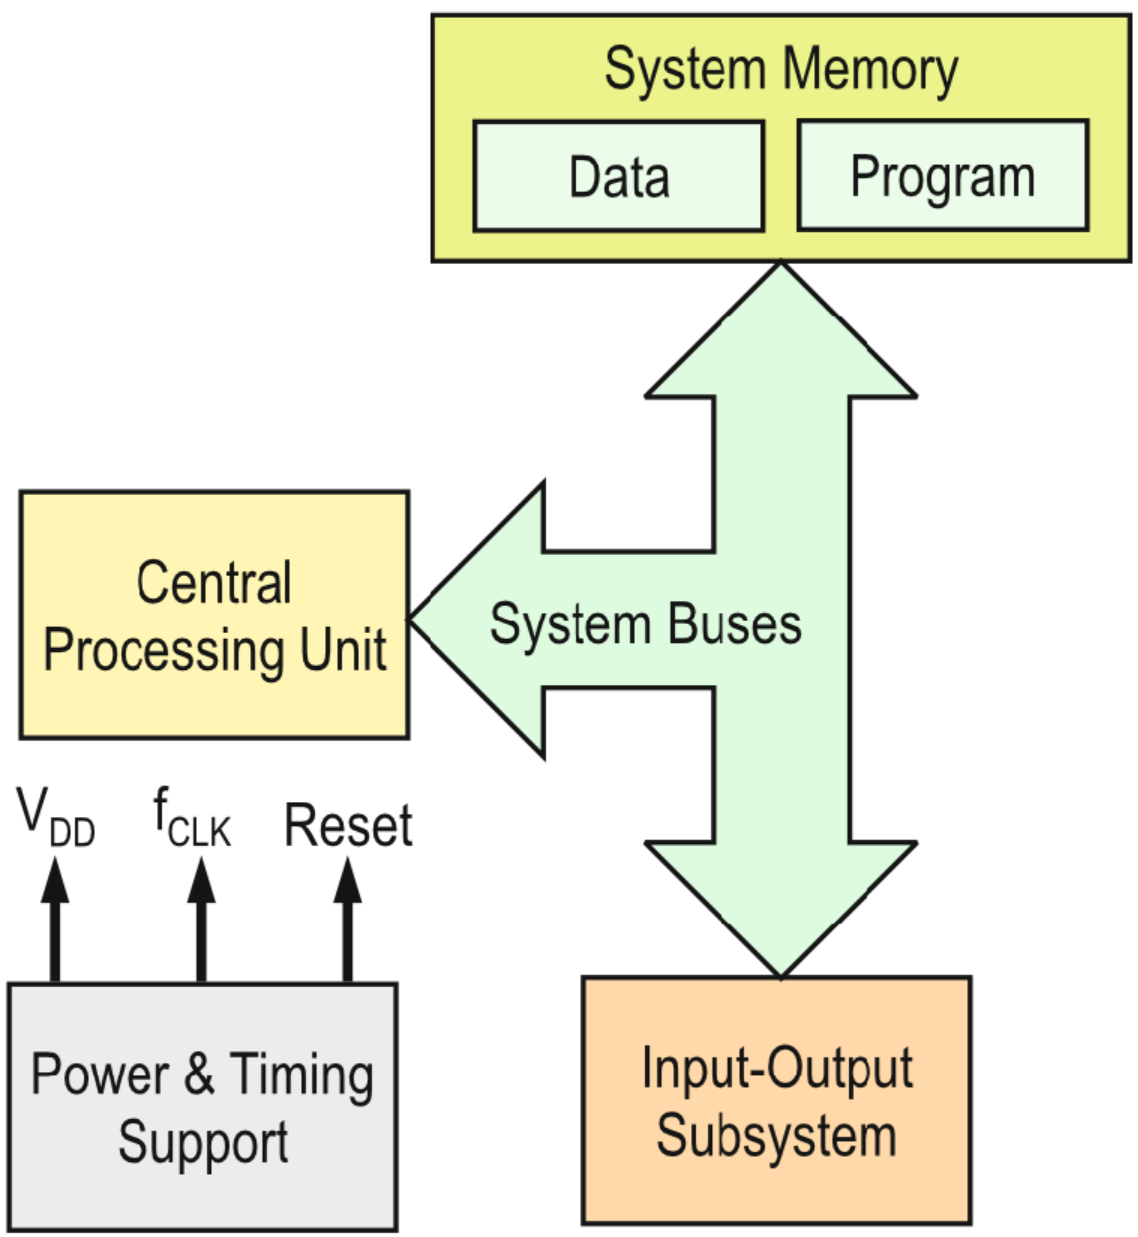
\includegraphics[width=\linewidth]{images/uCArchitecture}  
    \end{wrapfigure}
    
\begin{itemize}
    \item Central Processing Unit (CPU)
        \subitem Fetches, decodes and executes instructions from memory
    \item System Memory
        \subitem Program memory
        \subitem Data memory 
    \item Input-Output Subsystem
        \subitem Connect to the external world
    \item System Buses 
        \subitem Address bus
            \subsubitem Indicate address to be accessed
        \subitem Data bus
            \subsubitem carry data or instruction being transferred
        \subitem Control bus 
            \subsubitem reulate the activity in address \& data buses 
\end{itemize}
\subsection{Microcontroller vs. Microprocessors}
\begin{multicols}{2}
    \begin{minipage}{\linewidth}
        \textbf{Microprocessor(MPU)}
       \begin{itemize}
           \item Contain a Geberal Purpose CPU
               \subitem ALU, CU, Registers, BIL %Bus Interface Logic
           \item Require External Components to form a Basic System
               \subitem Buses
               \subitem Memory
               \subitem I/O Interface \& Devices
           \item Additionla Characteristics
               \subitem Architecture optimized for accelerating data processing
               \subitem Include elements to accelerate instruction execution  
        \end{itemize}
    \end{minipage}
    \begin{minipage}{\linewidth}
        \textbf{Microcontroller(MCU)}
        \begin{itemize}
            \item Contain a Microprocessor Core
                \subitem Usually less complex than that of an MPU
            \item Include memory and peripherals in a single chip
                \subitem Denominated $ computer-on-a-chip $ 
                \subitem Most MCUs do not provide external buses
            \item On-chip Memory
                \subitem Includes both, Program and Data-memory
            \item Typical Peripherals
                \subitem Timers
                \subitem I/O ports
                \subitem Data converters
        \end{itemize}     
    \end{minipage}
\end{multicols}
\begin{center}
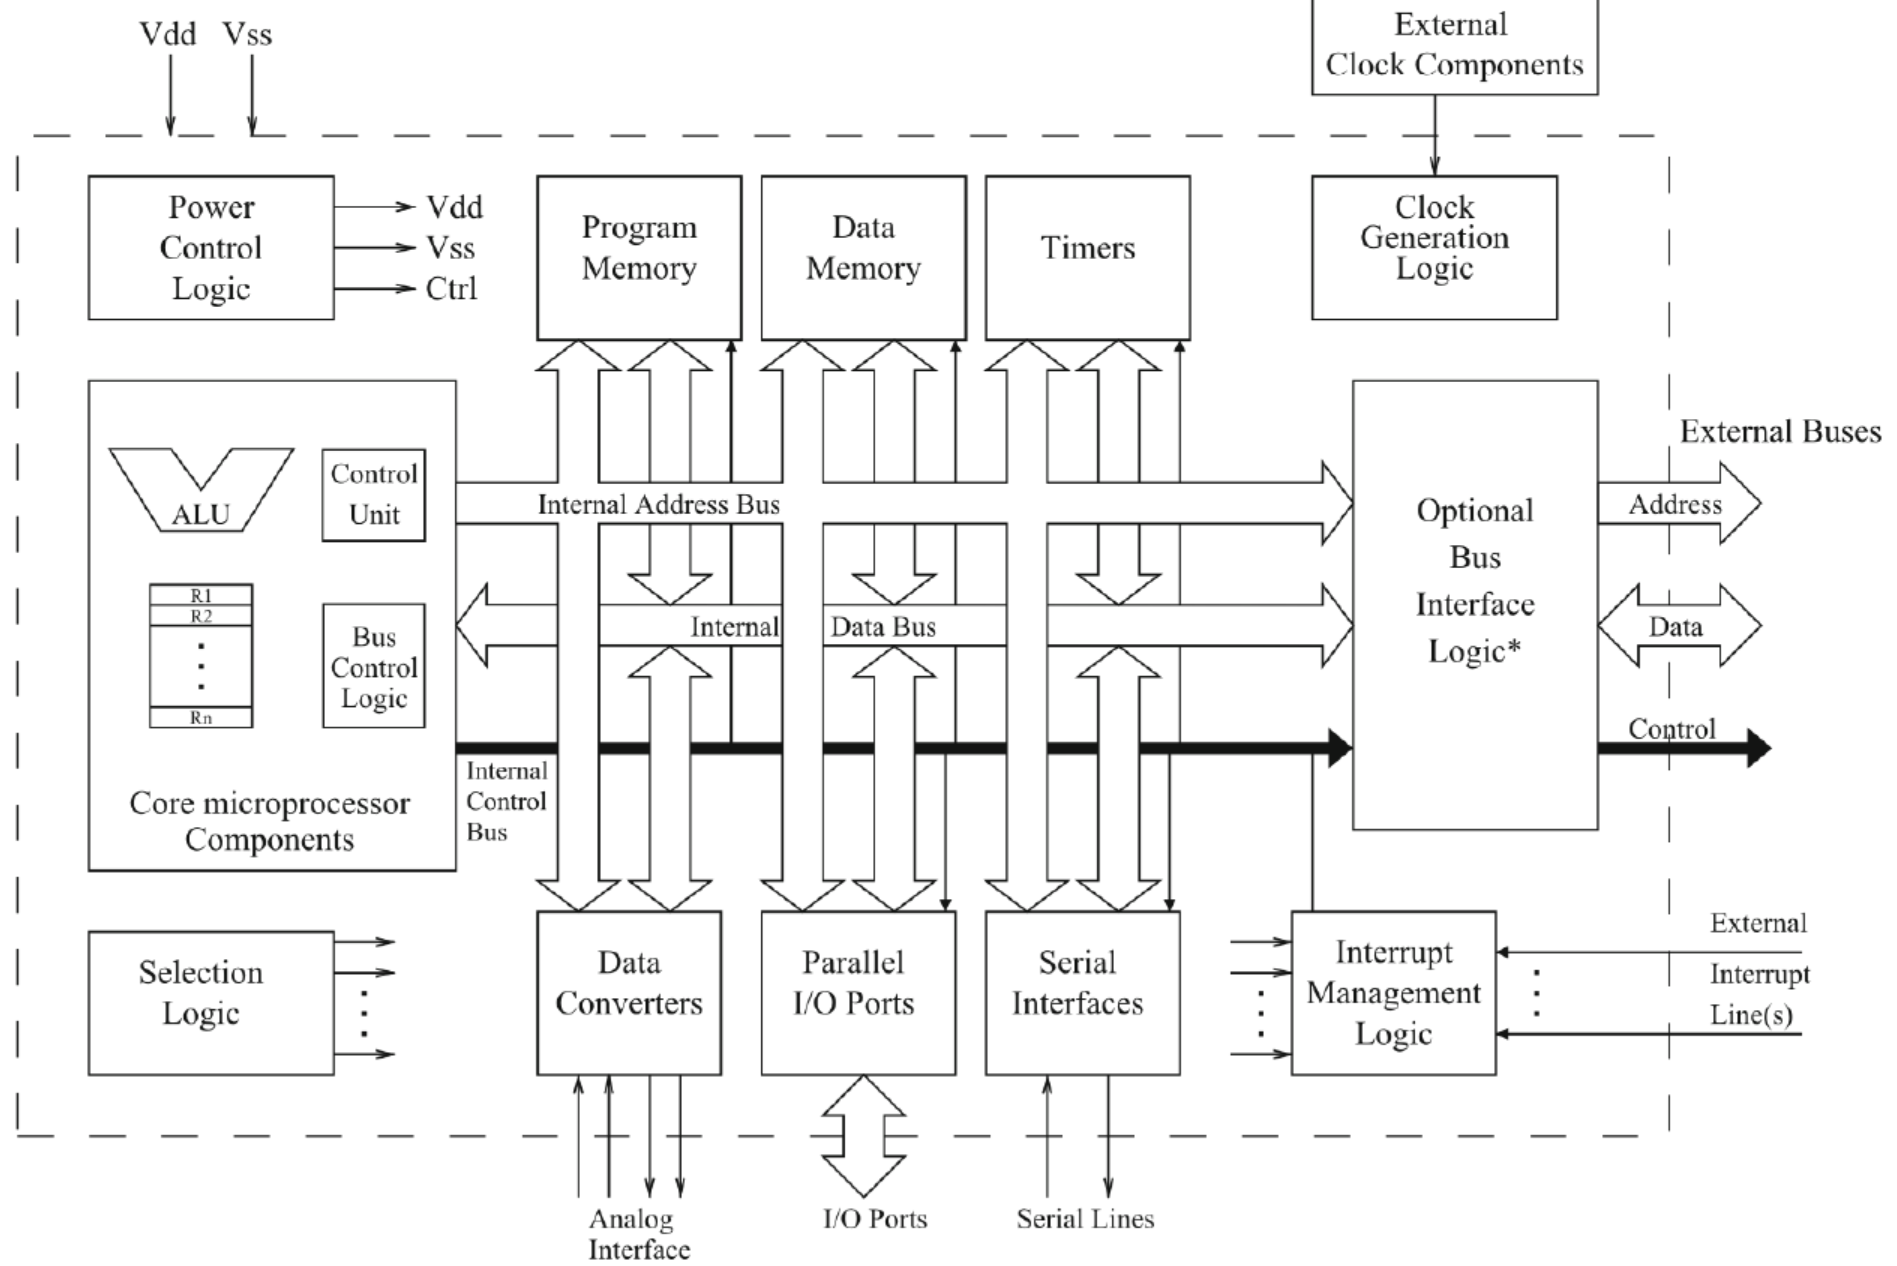
\includegraphics[width=0.6\linewidth]{images/mCStructure}
\end{center}
\subsection{RISC vs. CISC}
\begin{multicols}{2}
    \begin{minipage}{\linewidth}
        \textbf{CISC}\newline
        \textbf{Complex Instruction Set Computer}
        \begin{itemize}
            \item Variable length instructions
            \item Large instruction set
            \item Focuses in accomplishing as much as possible with each instruction
            \item Augments hardware complexity
            \item Simplifies programming
        \end{itemize}    
    \end{minipage}
    \begin{minipage}{\linewidth}
        \textbf{RISC}\newline
        \textbf{Reduced Instruction Set Computer}
        \begin{itemize}
            \item Fixed length insructions
            \item Short instruction set
            \item Focuses on simple instructions
            \item Simplifies the hardware structure
            \item Makes programming harder
          \end{itemize}      
    \end{minipage}
\end{multicols}

\subsection{Central Processing Unit}
\begin{multicols}{2}
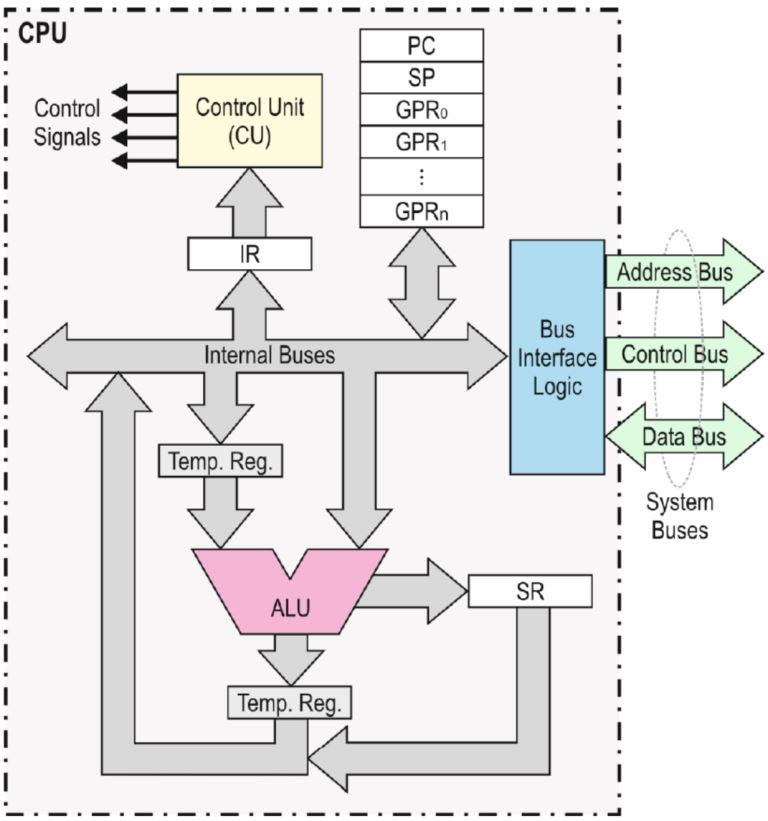
\includegraphics[width=\linewidth]{images/CPUComponents}
\begin{multicols}{2}
    \vspace*{-1cm}
\subsubsection{Control Unit (CU)}
    \textbf{Operations}
\begin{itemize}
    \item Governs the CPU working
    \item Cycles forever trough states:
        \subitem Fetch, Decode, Execute
\end{itemize}

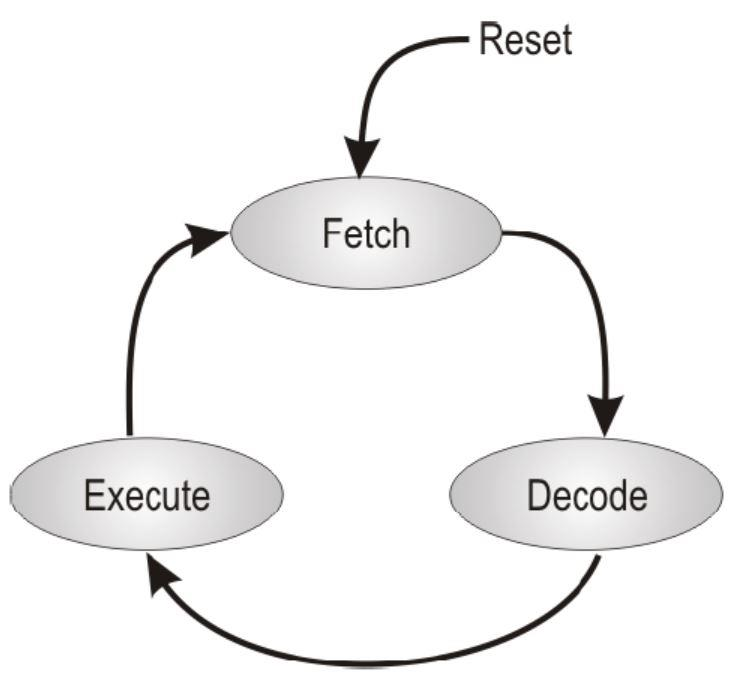
\includegraphics[width=0.85\linewidth]{images/FDELoop}
\end{multicols}

\subsubsection{Arithmetic Logic Unit (ALU)}
\begin{itemize}
    \item Performs Supported Logic and Arithmetic Operations
    \item 'Sets' the width of Databus and Registers
\end{itemize}

\subsubsection{Bus Interface Logic (BIL)}
\begin{itemize}
    \item Coordinates the interactioln between the internal buses and the system buses
\end{itemize}

\subsubsection{Registers}
    \begin{itemize}
        \item Provide temporary storage
        \item Volatile Contents
        \item General and Special Purpose Registers
    \end{itemize}
\end{multicols}

\subsection{General Purpose Registers vs Special Registers}
\begin{multicols}{2}
    \begin{minipage}{\linewidth}
        \textbf{General Purpose Register}
        \begin{itemize}
            \item Not tied to specific functions
            \item Can hold data, variables, or addresses
            \item Number of registers depend on CPU architecture
        \end{itemize}
    \end{minipage}
    \begin{minipage}{\linewidth}
        \textbf{Special Registers}
        \begin{itemize}
            \item Instruction Register (IR)
                \subitem Holds the current instruction 
            \item Programm Counter (PC)
                \subitem Holds the address of the next instruction to be fetched
            \item Stack Pointer (SP)
                \subitem Holds the address of the current top-of-stack 
            \item Status Regisrer (SR)
                \subitem Holds the current CPU Status (Flags)
        \end{itemize}
        
    \end{minipage}
\end{multicols}

\subsection{I/O Subsystem}
Convers all the components other than the CPU \& memory connected to the system buses
\begin{itemize}
    \item Timers and Watchdog timers
    \item Communication interfaces
    \item Analog to Digital Converter (ADC)
    \item Digital to Analog Converter (DAC)
    \item Development peripherals
\end{itemize}
\begin{multicols}{2}
    \begin{minipage}{\linewidth}
        \textbf{Memory mapped I/O}\newline
        Address spaace inside the momory space, uses same instructions used to access memory
    \end{minipage}
    
    \begin{minipage}{\linewidth}
        \textbf{I/O mapped I/O} \newline
        Separate address space, instrutions, and signals for I/O (rarley used in modern processors)
    \end{minipage}
\end{multicols}
\hspace{0.5cm}
\begin{multicols}{2}
    \begin{minipage}{\linewidth}
        Include lines to connect to the system buses, I/O device connection lines and a set of internal registers
        \begin{tabular}{ll}
            Control & to configure the operation of the device and interface  \\  
            Status & to allow inquires about the device and interface status  \\ 
            Data & for exchanging data with the device \\ 
        \end{tabular} 
    \end{minipage}
    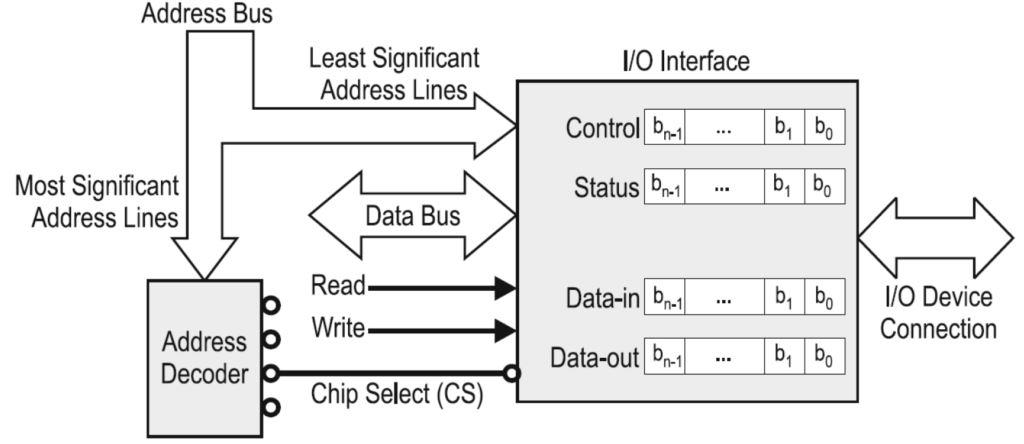
\includegraphics[width=0.9\linewidth]{images/IOAnatomy}  
\end{multicols}



\clearpage
